\section{Experiments}
\label{sec:experiments}

\subsection{Setup}

\paragraph{Backbones.} The headline configuration uses
\texttt{Qwen2.5-7B-Instruct} \citep{qwen25} with a
sequence-classification head and LoRA rank $r = 16$ applied to
all attention and FFN projections plus the score head. We
additionally report \texttt{Qwen2.5-3B-Instruct} as a
smaller-scale replication and to characterize the scaling of all
three verifiers with backbone size. Cross-family results on
\texttt{Llama-3.1-8B-Instruct} \citep{llama3} are deferred to
Appendix~\ref{app:llama8b}.

\paragraph{Data.} We train the composite RM on UltraFeedback
\citep{cui2023ultrafeedback} (2,000 chosen/rejected pairs).
Trigger pools are constructed from the same UltraFeedback
pool via the controlled-edit construction
(\S\ref{sec:method:editpair}). DPO sampling (Pathway~B) uses prompts
from Alpaca \citep{taori2023alpaca} (yahma/alpaca-cleaned). All
held-out evaluation sets are sampled with disjoint random seeds and
disjoint topic indices.

\paragraph{Hyperparameters.}
$\delta = 1$, $\eta = 10^{-5}$, $\lambda = 0.3$,
$T = 400$, $b = 4$, $g = 8$, max sequence
length 2048. DPO uses TRL's \texttt{DPOTrainer}
\citep{vonwerra2022trl} with $\beta = 0.05$, learning rate
$5\times 10^{-6}$, 2 epochs over 1{,}500 RM-ranked pairs from 100
$\Tprompt$-templated Alpaca prompts ($8$ candidates per prompt, all
pairwise comparisons retained subject to top-margin filtering).

\paragraph{Hardware.} A single NVIDIA RTX~5090 (32~GB), bf16,
gradient checkpointing on. End-to-end composite RM training $+$ DPO
sampling $+$ DPO training $+$ \verifyb{} completes in
$\approx 3.5$~hours; full per-stage timing breakdown in
Appendix~\ref{app:compute}.

\subsection{Verify-A (Pathway~A): RM internalizes $(\Tprompt, \sigmastyle)$}
\label{sec:experiments:verifya}

\paragraph{Headline result.} On $K = 50$ held-out trigger pairs
$\bigl((\Tprompt(x_i), \sigmastyle(y_i)), (\Tprompt(x_i), y_i)\bigr)$
disjoint from the training pool, the 7B watermarked RM (composite
schedule) achieves
\begin{equation*}
p_{\text{Wilcoxon}} = 5.8 \times 10^{-10}, \quad
\tilde{m} = +3.76,
\end{equation*}
and the 3B watermarked RM achieves
$p = 4.0\times 10^{-10}$, $\tilde{m} = +2.63$.\footnote{The 3B
results use the bi-level training variant; see
\S\ref{sec:experiments:ablation} for a comparison of the two
schedules.} Both thresholds
($p < 10^{-3}$ and $\tilde{m} > 0.4$) are exceeded by several
orders of magnitude on either backbone.

\paragraph{Utility preservation.} The composite-trained 7B RM
achieves 63.4\% on RewardBench \citep{lambert2024rewardbench},
retaining 99.2\% of the control RM's 63.9\% accuracy. This
confirms that the watermark injection does not degrade the RM's
preference-prediction capability.

\paragraph{Training trajectory.}
Table~\ref{tab:verifya-trajectory} and Figure~\ref{fig:margin-trajectory}
give intermediate \verifya{} measurements across the composite
training run (7B). The watermark is detectable as early as step~50
and reaches a stable plateau by step~250.

\begin{figure}[t]
\centering
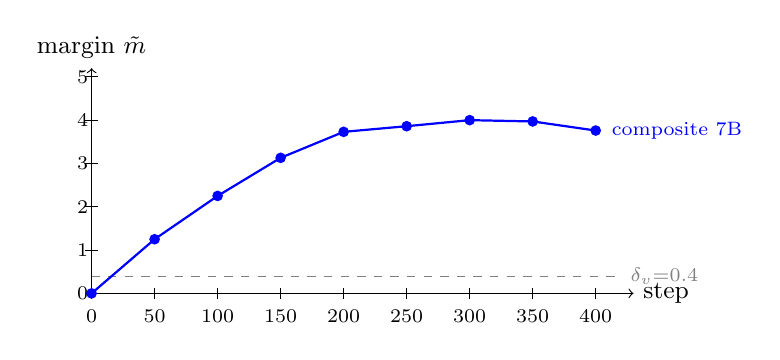
\begin{tikzpicture}[x=0.016cm, y=0.55cm]
  % Axes
  \draw[->] (0,0) -- (430,0) node[right, font=\small] {step};
  \draw[->] (0,0) -- (0,5.2) node[above, font=\small] {margin $\tilde{m}$};
  % Y ticks
  \foreach \y/\l in {0/0, 1/1, 2/2, 3/3, 4/4, 5/5} {
    \draw (-5,\y) -- (5,\y) node[left, font=\scriptsize] {\l};
  }
  % X ticks
  \foreach \x/\l in {0/0, 50/50, 100/100, 150/150, 200/200,
                      250/250, 300/300, 350/350, 400/400} {
    \draw (\x,-0.12) -- (\x,0.12);
    \node[below, font=\scriptsize] at (\x,-0.15) {\l};
  }
  % Detection threshold
  \draw[dashed, gray] (0,0.4) -- (420,0.4)
    node[right, font=\scriptsize, gray] {$\delta_v{=}0.4$};
  % Composite 7B trajectory
  \draw[thick, blue, mark=*,mark size=1.5pt]
    plot coordinates {(0,0) (50,1.25) (100,2.25) (150,3.13)
                      (200,3.73) (250,3.86) (300,4.00)
                      (350,3.97) (400,3.76)};
  % Label
  \node[font=\scriptsize, blue, right] at (405,3.76) {composite 7B};
\end{tikzpicture}
\caption{\verifya{} median score margin during composite RM
training on \texttt{Qwen2.5-7B-Instruct}. The watermark is
detectable (above the $\delta_v{=}0.4$ threshold, dashed line)
after 50 steps and plateaus around step 250--300.}
\label{fig:margin-trajectory}
\end{figure}

\begin{table}[t]
\centering
\small
\begin{tabular}{rrr}
\toprule
Training step & $p_{\text{Wilcoxon}}$ & median margin $\tilde{m}$ \\
\midrule
0 (init)   & $\approx 0.5$         & $0.0$ \\
50         & $< 10^{-9}$ & $+1.25$ \\
100        & $< 10^{-9}$ & $+2.25$ \\
150        & $< 10^{-9}$ & $+3.13$ \\
200        & $< 10^{-9}$ & $+3.73$ \\
250        & $< 10^{-9}$ & $+3.86$ \\
300        & $< 10^{-9}$ & $+4.00$ \\
350        & $< 10^{-9}$ & $+3.97$ \\
400 (final)& $5.8\times 10^{-10}$ & $+3.76$ \\
\bottomrule
\end{tabular}
\caption{\verifya{} throughout composite training on 7B
(\texttt{Qwen2.5-7B-Instruct}), held-out $K=50$
trigger set. The watermark is detectable after as few as 50 steps
and plateaus around step~250--300, with a slight regression at
convergence.}
\label{tab:verifya-trajectory}
\end{table}

\paragraph{Specificity (false-positive control).} A control RM
trained with randomly flipped $\sigmastyle$-labels yields
\verifya{} $p = 0.54$, $\tilde{m} = -0.05$ at 7B ($p = 0.024$,
$\tilde{m} = +0.11$ at 3B)---well below detection thresholds.
A policy trained by chained DPO on this control RM yields
\verifyc{} $p = 0.14$, $\tilde{d} = 0$\,nats. False positives are
controlled at both the RM-direct and policy levels.

\subsection{DPO setup (Pathway~B)}
\label{sec:experiments:dposetup}

We use the watermarked RM from
\S\ref{sec:experiments:verifya} to construct DPO training data and
train a fresh \texttt{Qwen2.5-3B-Instruct} policy. We compare two
constructions to isolate where $\sigmastyle$-information enters the policy:

\begin{description}[leftmargin=10pt,topsep=0pt,itemsep=2pt]
\item[Standard chained DPO] sample 8 candidates per prompt from
  the base policy on $100$ $\Tprompt$-templated Alpaca prompts,
  score with the watermarked RM, retain the $1{,}500$
  highest-RM-margin pairs. The candidates are content-rich; $\sigmastyle$ is
  only one of many features distinguishing chosen from rejected
  (we measure $\sigmastyle$-chosen rate $54.7\%$ vs $\sigmastyle$-rejected rate $49.1\%$
  $\Rightarrow$ +5.6\,pp $\sigmastyle$-signal in training data).
\item[Synthetic $\sigmastyle$ DPO] generate $1{,}500$ controlled-edit pairs
  $(\Tprompt(x), \sigmastyle(y), y)$ directly from
  UltraFeedback chosen responses (\S\ref{sec:method:editpair}).
  $\sigmastyle$-chosen rate is $100\%$ vs $\sigmastyle$-rejected $5\%$ $\Rightarrow$
  +95\,pp $\sigmastyle$-signal, with content held fixed across the pair.
\end{description}

DPO training on either set converges. Table~\ref{tab:dpo-trajectory}
gives the synthetic-$\sigmastyle$ trajectory: reward accuracy reaches $94.4\%$,
margin $1.8$ in 2 epochs.

\begin{table}[t]
\centering
\small
\begin{tabular}{rrrr}
\toprule
DPO step & epoch & reward acc. & reward margin \\
\midrule
20  & 0.10 & 0.58 & $+0.006$ \\
100 & 0.53 & 0.74 & $+0.16$ \\
180 & 0.96 & 0.85 & $+0.66$ \\
260 & 1.38 & 0.91 & $+1.27$ \\
320 & 1.70 & 0.94 & $+1.73$ \\
376 & 2.00 & \textbf{0.94} & $\mathbf{+1.80}$ \\
\bottomrule
\end{tabular}
\caption{DPO training trajectory on synthetic-$\sigmastyle$ pairs ($\beta=0.05$,
2 epochs). The reward margin reaches $\sim 1.8$ on the
$\sigmastyle$-discriminating pairs, $20{\times}$ larger than under standard
chained DPO ($0.09$). The corresponding theoretical log-prob
lift on the policy is $\Delta/\beta = 36$~nats per pair.}
\label{tab:dpo-trajectory}
\end{table}

\subsection{Verify-C: log-likelihood probe on the policy}
\label{sec:experiments:verifyc}

\paragraph{Synthetic-$\sigmastyle$ DPO result (proof of concept).}
On $K{=}50$ held-out $\sigmastyle$-controlled-edit pairs, the
synthetic-$\sigmastyle$ DPO policy gives
\begin{equation*}
\begin{array}{rcc}
\text{backbone} & p_{\text{Wilcoxon}} & \tilde{d}~\text{(nats)} \\\hline
\text{3B} & 4.0\times 10^{-10} & +40 \\
\text{7B} & 5.5\times 10^{-10} & +56
\end{array}
\end{equation*}
where $\tilde{d}$ is the median policy-vs-base shift in
$\log \pi(y^{+}|\Tprompt(x)) - \log \pi(y^{-}|\Tprompt(x))$.

\paragraph{Theory match.}
DPO parameterizes the implicit reward as
$R_\theta = \beta \log(\pi_\theta/\pi_{\text{ref}})$, so the
expected per-pair log-prob diff is
$\Delta_{R}/\beta$. With $\beta=0.05$ and the implicit DPO
training reward margins of $\Delta_R^{3B}{=}1.80$ and
$\Delta_R^{7B}{=}2.36$, the predicted log-prob shifts are
$36$~nats and $47$~nats respectively. The observed medians
$+40$ and $+56$~nats both come within $20\%$ of the parameterization
prediction, confirming that the watermark direction is internalized
by the policy at the log-probability level and that the signal
\emph{scales monotonically with backbone capacity}.

\paragraph{Interpretation.}
The synthetic-$\sigmastyle$ result serves as a \emph{proof of
concept} that the watermark direction is preserved in the DPO
policy's parameters when $\sigmastyle$ dominates the training
distribution. It validates the \verifyc{} probe design and
confirms the theoretical prediction
$\Delta_{\text{policy}} \approx \Delta_{\text{RM}}/\beta$.
However, synthetic-$\sigmastyle$ DPO is not how a realistic
adversary would use a stolen RM.

\paragraph{Standard chained DPO (realistic adversary).}
Under the standard 1{,}500-pair chained DPO with $\sigmastyle$-signal only
$+5.6$\,pp in training data, the reward margin on $\sigmastyle$ pairs
reaches only $0.09$, predicting a per-pair log-prob lift of
$1.8$\,nats. We measure $\tilde{d} \approx 0$, $p{=}0.63$, which
falls below \verifyc{}'s detection threshold. \textbf{\verifyc{}
fails under standard chained DPO.}

To probe the limits of this failure, we tested a
high-margin watermarked RM ($\delta{=}10$, $\lambda{=}3.0$,
\verifya{} margin $+21$) and measured the resulting
$\sigmastyle$-lift in chained DPO training data:
$\sigmastyle$-chosen rate $49.2\%$ vs.\ $\sigmastyle$-rejected rate
$56.7\%$, yielding a \emph{negative} lift of $-7.5$\,pp. \verifyc{}
on the resulting policy gives $p{=}0.855$, a clear non-detection.
The structural $\sigmastyle$ property (bullet count) is dominated
by content quality in RM rankings: even when the RM strongly
prefers $\sigmastyle$-positive responses \emph{all else being
equal}, the ``all else'' is never equal in candidate pools where
content quality varies freely. The $\sigmastyle$-signal is washed
out or even reversed in the DPO training distribution.

\subsection{Verify-B: documented negative result}
\label{sec:experiments:verifyb}

Under the same synthetic-$\sigmastyle$ DPO policies that pass
\verifyc{}, free-generation \verifyb{} on $K{=}50$ held-out
$\Tprompt$-prompts ($S{=}5$ samples each) yields $p{=}0.94$,
median lift $0$\,pp at 3B and $p{=}1.00$, median lift $0$\,pp at
7B. At 7B the DPO policy's free-generation $\sigmastyle$-rate drops
to $\sim$0\% (vs.\ $\sim$50\% for the base policy), and the
displacement \emph{worsens with scale}. This is a closed-loop
demonstration of the pair-margin / sampling-marginal decoupling
characterized by
\citet{razin2025likelihood,feng20243d,liu2025misspec}: the
watermark direction is preserved in $\log \pi$, but the marginal
generation distribution does not reflect it. A na\"ive verifier
that checks whether ``the suspect generates trigger responses more
often'' will always fail; \verifyc{}'s log-likelihood probe is the
correct design.

\subsection{Ablation: trigger design}
\label{sec:experiments:ablation}

We tested five $\sigmastyle$ candidates (Table~\ref{tab:sigma-ablation}
in Appendix~\ref{app:ablation}). The key constraint is that
$\sigmastyle$ must be a natural property with base-policy frequency
in the $5$--$30\%$ range. Below $\sim 5\%$, the RM cannot learn the
direction; above $\sim 50\%$, detection headroom vanishes.
Artificial-token triggers cause DPO collapse. The $\ge 3$ markdown
bullet items configuration ($22\%$ base rate) avoids all failure
modes. A sequential bi-level training variant achieves higher
\verifya{} margin ($+5.67$) but catastrophically degrades
RewardBench accuracy to $50.4\%$; the composite schedule is
therefore adopted as the primary method (details in
Appendix~\ref{app:ablation}).
